\subsection{Regression Model}
To answer the research question of this paper, the effect of depression on obesity, the following basis of regression model was used:


\[
\text{Obese} = \beta_0 + \beta_1 \cdot \text{CESD} + \beta_2  \cdot \text{Male} + \beta_3 \cdot \text{Male} \cdot  \text{CESD}+ \beta_4 \cdot \text{Smoked} + \beta_5 \cdot \text{Male} \cdot \text{Smoked} +\delta \cdot \text{wave}  + \xi \cdot \chi + \epsilon
\label{eq:model1}
\]

Where wave is a vector of dummies telling in which wave the observation is and $\xi$ is composed of the controls education level, age and smoking situation of the spouse.

We then computed this model using 3 regressions types: 
\begin{itemize}
\item A linear regression
\item A linear regression using the spouse's CESD score as instrument for CESD  score and the spouse's interaction for the interaction effect. (gender times CESD score)
\item The above regression using an instrumental probit instead of the linear regression
\end{itemize} 

Auxiliary regressions were also performed using weight problems, overweight and morbidly obese as the explained variable instead of obese.

\subsection{Main results}

Table \ref{tab:obese} clearly shows a strongly positive influence of the depression score on the probability of becoming obese (almost $5\%$ at the mean). What is also worth noting is that females are severely more affected by this (being a male more than halves the coefficient, but still keeps it significantly different from zero) even though males are more likely to be obese in the baseline situation ($6.5\%$ in the non-depressed case).

It is also worth noting that older people are less likely to be obese but this result suffers from endogeneity (being obese decreases the life expectancy) and also from the age distribution of the database (only takes the older part of the population into account) and since it was not the focus of the study, trying to improve the identification of this effect through a better functional form did not make sense. The age of the spouse does not have any significant effect.

Having smoked strongly decreased the probability of being obese ($-15\%$) and the effect did not seem to vary through sexes, while the smoking situation of the spouse did not have any significant effect.

Regarding the controls, as it can be seen in table \ref{tab:wave} and \ref{tab:educ}, the wave (thus the year of the observation) has a positive influence on the probability of being obese and a higher education reduces that probability.

\subsection{Strong Instrument}
The chosen instruments are very strong as was observed with the Cragg-Donald Wald F statistic of over 2000 in all the regressions.

It is interesting to observe that the use of instruments actually increases the amplitude of the coefficient compared to the regression with the endogenous regressor. As it can be seen in table \ref{tab:bias}, the simplest regression roughly keeps the same coefficients as the complete one. The simpler regression allows to compute the direction of the bias:  reducing the bias by using an instrument increased the coefficient, which implies that the bias was negative, thus the regressor (depression score) is negatively correlated with the errors which suggests a negative effect of obesity on depression using (with $\alpha_1$ the effect of depression on obesity and $\alpha_2$ the effect of obesity on depression):
\[
\text{Cov}(x, u) = \frac{\alpha_2}{1 - \alpha_1 \alpha_2} \sigma_\epsilon^2
\]
conditional on $\alpha_1 \alpha_2 < 1$ which seems plausible since $\alpha_1$ is very small.

\subsection{Auxiliary results}

The coefficient of interest behave similarly in all 4 cases and it can also be noted that the ivreg and the marginal effects of the iv profit are very similar suggesting that we are in the middle of the distribution (in the linear part). The only situation where there is a visible difference between the coefficient when comparing ivreg with ivprobit (however not significant) is in the morbidly obese case where we only have a small percentage of the population in one category thus putting the regression far from the linear part at the center.

The behaviour of the coefficients of interest can be seen in figure \ref{fig:results} and  \ref{fig:results2} :

\begin{figure}[H]
\makebox[\textwidth][c]{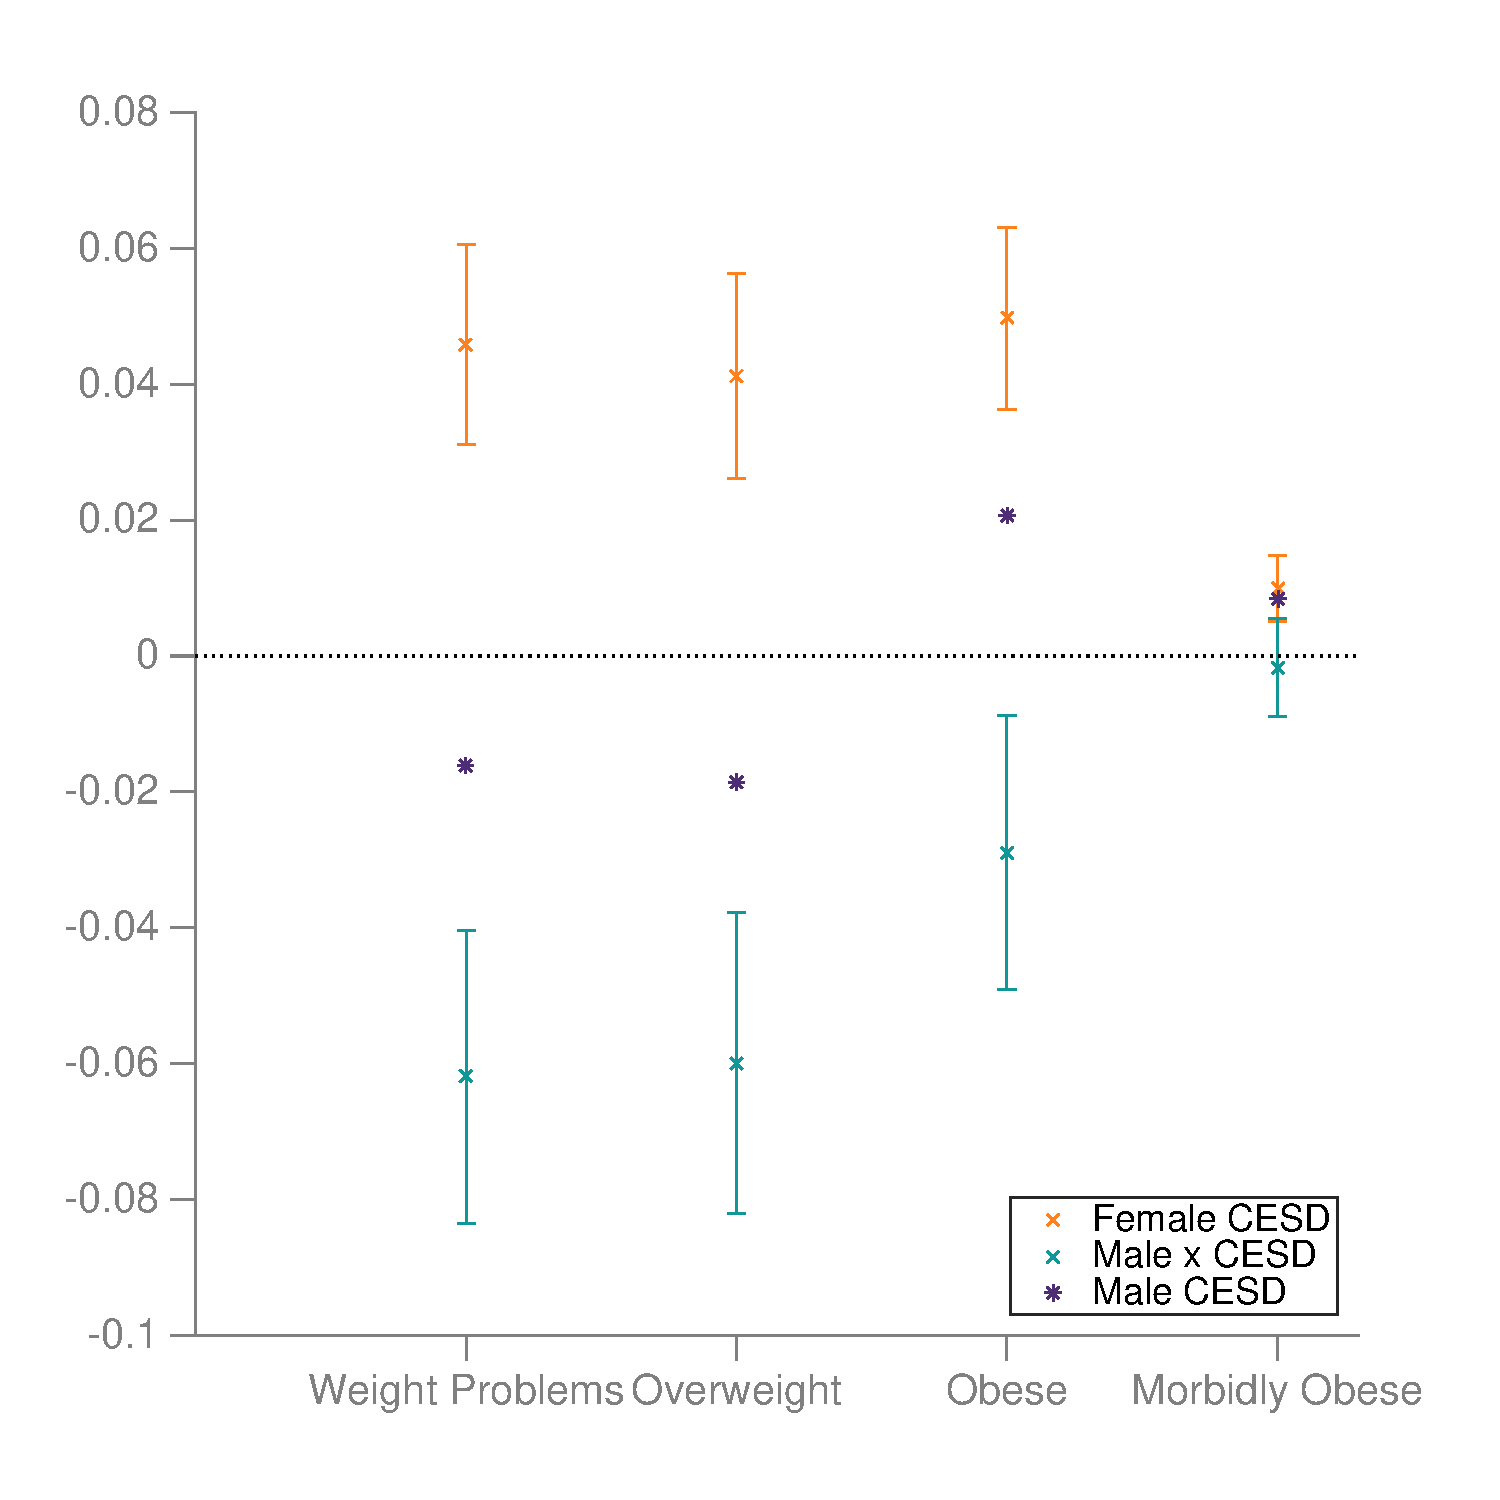
\includegraphics[width=0.6\paperwidth]{../proj/matlab/1.pdf}}
\caption{Visual representation of the obtained coefficients for CESD and both sexes}
\label{fig:results}
\end{figure}

As it can be seen, the effect of depression on being overweight or obese in female is very strong while being way lower (even changing sign in the broader categories) for males. However it is interesting to see that this difference disappears when looking at the probability of being morbidly obese where the sex does not play a role anymore.

Finally, the gender does not change the effect of smoking for any dependent variable.